\documentclass[11pt,a4paper]{article}
\usepackage{graphicx}
\usepackage{float}
\usepackage[authoryear]{natbib}
\usepackage{amsmath, amsthm, amssymb}
\usepackage{amsfonts}
\usepackage{makeidx}
\usepackage{lmodern}
\usepackage{grffile}
\graphicspath{ {figures/} }
\usepackage{array}
\usepackage{tocloft}
\usepackage{mathrsfs}
\usepackage[final]{pdfpages}
\usepackage{fancyhdr}
\usepackage{xcolor}
\usepackage{url}
\usepackage[colorlinks = true,
            linkcolor = blue,
            urlcolor  = blue,
            citecolor = blue,
            anchorcolor = blue]{hyperref}

\usepackage[left=2cm,right=2cm,top=2cm,bottom=2cm]{geometry}
\linespread{1}

\setlength{\headheight}{14pt} 
\title{Professional Development Plan}
\author{Pierre Le Roux}
\pagestyle{fancy}
\lhead{Pierre Le Roux}
\chead{Professional Development Plan}
\rhead{u13112262}

\begin{document}

	\begin{titlepage}
		
\includegraphics[width=\textwidth]{Extra/Front_Page.jpg}
	\end{titlepage}
	
	\pagebreak
	
	\pagenumbering{arabic}
	\setcounter{page}{1}
	
	\section{Purpose}
		The purpose of this plan is to ensure that all requirements in terms of ECSA outcomes are met, in the minimum amount of time of five years, by future candidate engineer Mr Pierre Le Roux (13112262) which will be referred to in this paper as FCE.
		The plan will cover the following:
		
		\begin{enumerate}
		\item	Registering at ECSA as a Professional Industrial Engineer
		
		\item	Completing one five year cycle of Continuous Professional Development (CPD)
		\end{enumerate}
		
		This plan isn't perfect and as circumstances change the plan will be rescheduled accordingly while still ensure that the FCE achieves said outcomes.
		
	\section{Directions}
		During the FCE's studies automation, simulation, operations research, processes and production automation peaks his interest. 
		The FCE's final year project , Improving FlySafair's Crew Scheduling, is an operations research project which combines programming, heuristics and modelling to create a more automated system the insures to generate a more optimal schedule for FlySafair.
		
	
	\section{Commitments}
		The FCE's has not commitments to a third party in terms of completing his B.Ing. degree.
		While it is fortunate that the FCE doesn't have any contractual requirement in terms of employment, but on the other hand the FCE will need to find employment to ensure he can complete the requirements in terms of the eleven ECSA outcomes and completing activities for CPD credits - Developmental, work-based and individual.
	
	\section{CDP To Achieve Professional Registration}
		If the FCE passes all his module this year he will graduate at the end of 2016.
		The FCE hopes that FlySafair would provide work for him based on the results of his final year project.
		Concerning the FCE's interests the following directions, but not limited to, are available:
		
		\begin{enumerate}
		\item	\textbf{Automation and Control} in decision support mechanisms
		
		\item	\textbf{Operations Research} in logistics
		
		\item	\textbf{Processes} in service industries
		
		\item	\textbf{Robotics and Production} in manufacturing industries
		
		\end{enumerate}
		
		Development in any of the above field is acceptable according to (ECSA \citeyear{ECSA_2013a}) as it is specific to the industrial engineering field. With FlySafair \textbf{Automation and Control} and \textbf{Operations Research} will be developed over a period of 36 months to comply with outcomes as stated in (ECSA \citeyear{ECSA_2012a}).
		
	\subsection{ECSA's Eleven Competency Standards}
		In figure \ref{fig: ECSA}, ECSA's eleven outcomes are summaries as stated in (R-08-PE \citeyear{ECSA_2012b}). 
		Theses consists of five main groups:
		
		\begin{itemize}
		
		\item[]	\textbf{Group A:} Knowledge-based Engineering Problem Solving (Outcomes 1, 2, 3)
			

		\item[]	\textbf{Group B:} Managing Engineering Activities (Outcomes 4, 5)

		\item[]	\textbf{Group C:} Risk and Impact Mitigation (Outcomes 6, 7)

		\item[]	\textbf{Group D:} Exercising Judgement and Taking Responsibility (Outcomes 8, 9, 10)

		\item[]	\textbf{Group E:} Developing Own Competency (Outcome 11)
				
		\end{itemize}

		\begin{figure}[H]
		\centering
		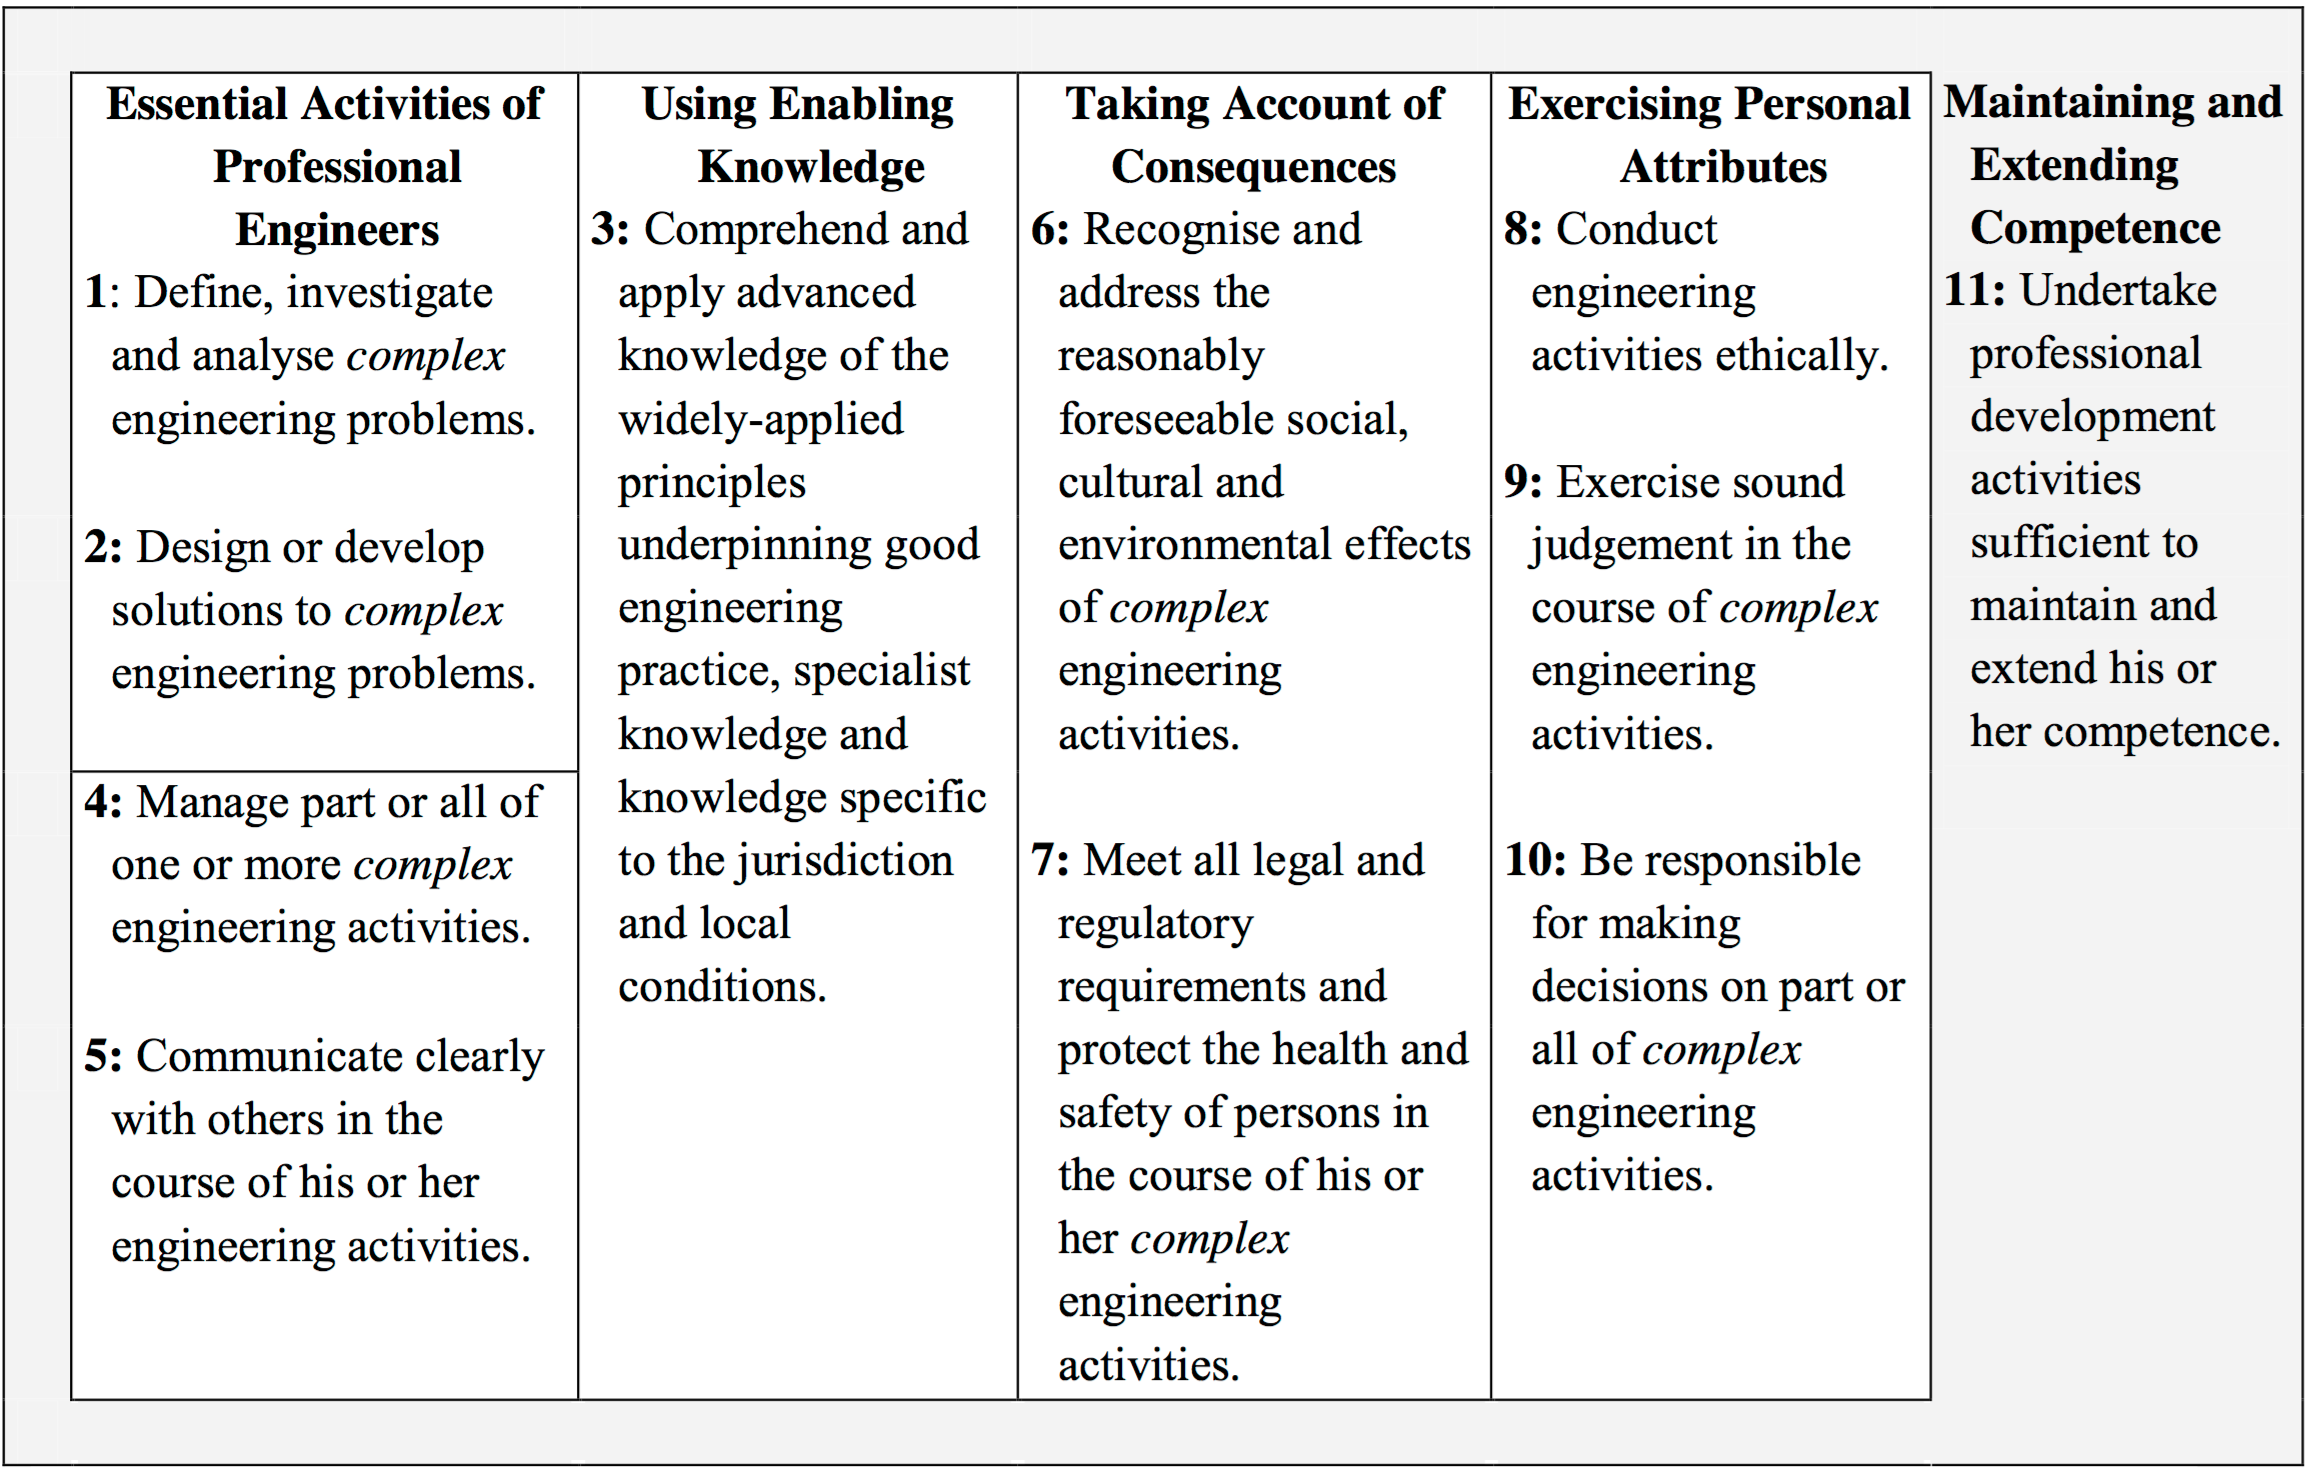
\includegraphics[width=\textwidth]{Extra/ECSA_Outcomes.png}
		\caption{Nested ECSA Outcomes for Registration as a Professional Engineer}\label{fig: ECSA}
		\end{figure}

	\begin{itemize}
	
	\item[\textbf{A}]
		To achieve outcome one to three, the FCE is considering a career in Operations Research which will, if accepted, develop knowledge-based Engineering Problem Solving in this field (ACSA \citeyear{ECSA_2012a}). 
		Doing postgraduate studies at ECSA accredited universities this knowledge can be expanded even further.
	
	\item[\textbf{B}] 
		Outcomes four and five, is developing and managing responsibilities in executing the tasks, projects and assignments.
	Theses responsibilities range from limited to full responsibility. During this phase the FCE can do extra accredited courses in project management to enhance his communication and managing skills so that he will use his resources, systems, people, money and process better.
	
	\item[\textbf{C}] 
		Operations Research:
	
		\begin{enumerate}
		\item	Possible optimal solutions may eliminate people's jobs.
	
		\item	Designing process to run at their maximum output can sometimes lead to failures in components which can endanger people.
		\end{enumerate}
	
	These and other requirements needs to be accounted for by the FCE to ensure that outcome six and seven is met and that the impacts of his engineering activities are optimised between man, money and machine.
	Accounting for the effect of his implementations both over the short and long period is important to achieve said outcomes.
	
	\item[\textbf{D}]
		The FCE will conduct himself ethically in all aspect and at minimum to that of the Code of Conduct, (ECSA \citeyear{ECSA_2013b}).
		While doing project and having more responsibility the FCE will taking risk factors into account when making decisions.
		Taking those decisions in complex engineering activities require understanding, sound judgment and taking responsibility for all outcomes of significant parts.
	
	\item[\textbf{E}] 
		During the process of becoming a Professional Engineer the FCE will undertake development activities to ensure that he stays his state-of-the-art competence. These activities consist, but isn't limited to:
		
		\begin{enumerate}
		
		\item	Being a SAIIE member
		
		\item	Taking accredited ACSA courses and conferences similar to SAPICS 2016, (SAIIE \citeyear{SAIIEa})
		
		\item	Attending postgraduate studies in the field of interest.
		
		\item	By working 800 hours per year during the candidate phase.
		
		\end{enumerate}
	
	\end{itemize}	
	
	\subsection{Tracking Process and keeping Record}
		To ensure that all area of ECSA outcomes are accounted for the FCE will keep record and track his process during his candidate phase. This will include the following:
		
	\begin{enumerate}
	
	\item	Submitting standard ECSA Training and Experience reports and keeping track of his daily activities.
			As he completes projects and assignments he will ask approval from his mentors and supervisors before submitting the above mentioned reports. 
			
	\item	By the end of the third year, the FCE will consult with he mentor and then create the required documents to apply for the Professional Engineering registration.
	
	\item	The FCE is granted registrations as a Professional Engineer if all the ECSA requirements are met. 
	This process will happen within six months of his submission for registration.
	\end{enumerate}
	
	\section{Full CPD Cycle as a Registered Professional Engineer}
	As required by ECSA (\citeyear{ECSA_2013c}), the Continuing Professional Development (CPD) for a single cycle, five years, is shown below in tables \ref{tab: Minimum} and \ref{tab: Recommended}. The total is calculated as shown below:
	
	\begin{equation}\label{eq:1}
		\begin{array}{c}
			\text{\textbf{Total}} = \displaystyle\sum\limits_{y=1}^{5} \displaystyle\sum\limits_{cat=1}^{3} \textbf{Credit}_{y, cat}
		\end{array}
	\end{equation}
	
	\subsection{Minimum Requirement Scenario}
	
	\begin{table}[H]
\centering
\caption{Minimum Requirement of a CPD Cycle}
\label{tab: Minimum}
\begin{tabular}{cl|c|c|c|c|c|r}
\cline{3-7}
\multicolumn{1}{l}{}           &                                       & \multicolumn{5}{l|}{Yearly Planned Credits} & \multicolumn{1}{l}{}                   \\ \hline
\multicolumn{1}{|l|}{Category} & Activity                              & Y1      & Y2     & Y3     & Y4     & Y5     & \multicolumn{1}{r|}{\textit{Subtotal}} \\ \hline
\multicolumn{1}{|c|}{1}        & Attending Courses and Conferences     & 2       & 2      & 2      & 2      & 2      & \multicolumn{1}{r|}{10}                \\ \hline
\multicolumn{1}{|c|}{2}        & Engineering Work (800 hours per year) & 2       & 2      & 2      & 2      & 2      & \multicolumn{1}{r|}{10}                \\ \hline
\multicolumn{1}{|c|}{3}        & Being a SAIIE Member                  & 1       & 1      & 1      & 1      & 1      & \multicolumn{1}{r|}{5}                 \\ \hline
\multicolumn{2}{|r|}{$\sum$}                                              & 5       & 5      & 5      & 5      & 5      & \multicolumn{1}{r|}{\textbf{25}}       \\ \hline
\end{tabular}
\end{table}


	\begin{equation}\label{eq:2}
		\begin{array}{c}
			\text{\textbf{Total}} = \displaystyle\sum\limits_{y=1}^{5} \displaystyle\sum\limits_{cat=1}^{3} \textbf{Credit}_{y, cat} = \displaystyle\sum\limits_{y=1}^{5} (2 + 2 + 1) = 25
		\end{array}
	\end{equation}

		The plan shown in table \ref{tab: Minimum} is good but it doesn't account for the fact that you might get busier as time progresses and then if you don't attend courses in the fourth and fifth year you'll not be able to reach the needed score of 25. Thus a more realistic plan was created to account for doing more in the initial stages.
	
	
	\subsection{Recommended Scenario}
	
	\begin{table}[H]
\centering
\caption{Recommended Scenario of a CPD Cycle}
\label{tab: Recommended}
\begin{tabular}{cl|c|c|c|c|c|r}
\cline{3-7}
\multicolumn{1}{l}{}           &                                       & \multicolumn{5}{l|}{Yearly Planned Credits} & \multicolumn{1}{l}{}                   \\ \hline
\multicolumn{1}{|l|}{Category} & Activity                              & Y1      & Y2     & Y3     & Y4     & Y5     & \multicolumn{1}{r|}{\textit{Subtotal}} \\ \hline
\multicolumn{1}{|c|}{1}        & Attending Courses and Conferences     & 6       & 5      & 4      & 0      & 0      & \multicolumn{1}{r|}{17}                \\ \hline
\multicolumn{1}{|c|}{2}        & Engineering Work (800 hours per year) & 2       & 2      & 2      & 2      & 2      & \multicolumn{1}{r|}{10}                \\ \hline
\multicolumn{1}{|c|}{3}        & Being a SAIIE Member                  & 1       & 1      & 1      & 1      & 1      & \multicolumn{1}{r|}{5}                 \\ \hline
\multicolumn{2}{|r|}{$\sum$}                                           & 9       & 8      & 7      & 3      & 3      & \multicolumn{1}{r|}{\textbf{32}}       \\ \hline
\end{tabular}
\end{table}

	\begin{equation}\label{eq:3}
		\begin{array}{c}
			\text{\textbf{Total}} = \displaystyle\sum\limits_{y=1}^{5} \displaystyle\sum\limits_{cat=1}^{3} \textbf{Credit}_{y, cat} = \displaystyle\sum\limits_{y=1}^{5} (cat=1 + cat=2 + cat=3) = 32
		\end{array}
	\end{equation}

	In table \ref{tab: Recommended} the scenario is that in the first three years the FCE has acquired enough points so that in the fourth and fifth year if something goes wrong and he has to work more and cannot go to conferences or course that he still has enough point in accordance with ECSA.
	
	\pagebreak
		
	\bibliographystyle{plainnat}
	\bibliography{References}				

\end{document}
